\section{Client}
Πέρα από τον Server όπως προαναφέρθηκε, το 2ο μέρος της εφαρμογής είναι ο Client. Ο Client είναι το σύστημα που θα καταναλώσει τα δεδομένα από τον Server και θα τα εμφανίσει με έναν προσιτό και κατανοητό τρόπο στον χρήστη. Ο Client δομήθηκε με την χρήση της βιβλιοθήκης React του CoreUI και του Redux Framework.

Η React είναι η κεντρική βιβλιοθήκη που χρησιμοποιήθηκε και όλα τα άλλα συστήματα αλληλεπιδρούν με αυτήν. Το Redux χρησιμοποιήθηκε για την διαχείρισή της κατάστασης της εφαρμογής και το CoreUI για τα γραφικά της. Πέρα από αυτές τις κύριες τεχνολογίες χρησιμοποιήθηκε επίσης η βιβλιοθήκη Highcharts για τα γραφήματα, τα εικονίδια της βιβλιοθήκης CoreUI και FontAwesome, η βιβλιοθήκη lodash για την ευκολότερη διαχείρισή των Javascript Objects, και κάποιες άλλες μικρότερες βιβλιοθήκες για την βελτίωση της αισθητικής του γραφικού περιβάλλοντος και την ευκολότερη διαχείριση των συστημάτων του Frontend. 

Ο Client στην ουσία είναι μια Web εφαρμογή και αποτελείται από 2 κομμάτια. Το πρώτο είναι το Dashboard, το οποίο εμφανίζει όλα τα δεδομένα που προσφέρει ο Server. Το δεύτερο κομμάτι είναι η σελίδα παρακολούθησης των στατιστικών των υπηρεσιών. Η αρχιτεκτονική του Client είναι SPA, που σημαίνει ότι υπάρχει μόνο μια σελίδα και το περιεχόμενο της σελίδας αλλάζει με την React.

Η React λειτουργεί με Components. Component είναι ένα στοιχείο το οποίο εμφανίζεται κάπου μέσα στην Web εφαρμογή. Η Συνολική εφαρμογή αποτελείται από πολλά Components τα οποία συνδυάζονται και εμφανίζονται μαζί για να φανεί το τελικό αποτέλεσμα. Τα Component είναι ένας έξυπνος τρόπος δόμησης μιας Web Εφαρμογής καθώς μπορούν να ξανά χρησιμοποιηθούν σε πολλά μέρη της εφαρμογής. Με αυτόν τον τρόπο έχοντας ένα αρχείο για κάθε Component γίνεται πιο ξεκάθαρη η δομή της εφαρμογής και ο τρόπος που λειτουργεί το κάθε Component, και καθίσταται ευκολότερη η συντήρηση και αλλαγή κώδικα αλλά και η αντιμετώπιση σφαλμάτων. 

Η Βασική δομή αποτελείται από το Header Component, το Router Component και το Footer Component όπως φαίνεται στο σχήμα \ref{wire:main}. Το Header αποτελείται από μια εικόνα, το λογότυπο της εφαρμογής, στα αριστερά και ένα εικονίδιο με εικόνα ένα γρανάζι στα δεξιά το οποίο επιτρέπει την αλλαγή γλώσσας, την είσοδο στην εφαρμογή και σε περίπτωση που ο χρήστης είναι ήδη εξουσιοδοτημένος σαν διαχειριστής, έναν σύνδεσμο στο πάνελ διαχείρισης. Το Footer αναγράφει την ημερομηνία κατασκευής της εφαρμογής καθώς και το όνομα του δημιουργού στα αριστερά, και στα δεξιά αναγράφει τις κύριες τεχνολογίες που χρησιμοποιήθηκαν για να γίνει η εφαρμογή. Το Router από την άλλη είναι μια περιοχή η οποία θα αλλάζει ανάλογα με το τι χρειάζεται να εμφανιστεί κάθε φορά. Τα περιεχόμενο που αλλάζουν μέσα στο Router μπορούν να χαρακτηρησούν σαν σελίδες. Οποιαδήποτε αναφορά σε "σελίδες" αργότερα, έκτος αν διευκρινιστεί κάτι άλλο, θα αφορά τις "εικονικές" σελίδες που αλλάζει το Router.

\begin{figure}[h]
  \centering
  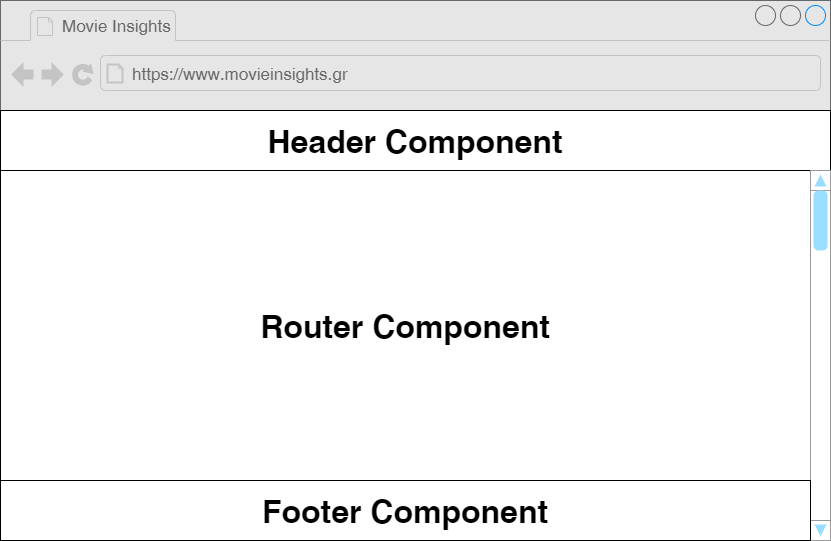
\includegraphics[width=145mm]{Chapters/5 - Architecture/Client/Images/main_struct.png}
  \caption{Βασική διάταξη Web εφαρμογής}
  \label{wire:main}
\end{figure}

Η εφαρμογή αυτή επίσης έχει Modules. Η έννοια Module στην React δεν υπάρχει σε αντίθεση με κάποιο άλλο Web Framework όπως η Angular, αλλά για αυτήν την εφαρμογή στην ουσία ορίζει μια λειτουργία και ομαδοποιεί όλα τα Components αυτής της λειτουργίας μαζί. 

Η αρχιτεκτονική του Router είναι δυναμική καθώς επιτρέπει κάθε Module να ορίζει το δικό της Router με τα δικά του Routes. Υπάρχουν 4 ειδών Routes. Το πρώτο είναι το απλό Route που όταν αλλάζει η διεύθυνση στην γραμμή εισαγωγής διεύθυνσης σελίδας αλλάζει και το περιεχόμενο που συνήθως κάθε route είναι και μια σελίδα. Το δεύτερο ονομάζεται PrivateRoute και επιτρέπει την πρόσβαση στην δηλωμένη διεύθυνση μόνο αν ο χρήστης έχει κάνει Login, και είναι εξουσιοδοτημένος για να δει την σελίδα που ζητάει. Το τρίτο Route είναι ένα RedirectRoute που όταν πηγαίνει ο χρήστης εκεί τον ανακατευθύνει σε ένα αλλο Route, και το τέταρτο Route είναι ένα Route που ενεργοποιείται όταν η διεύθυνση που έχει δοθεί δεν ανταποκρίνεται σε κανένα δηλωμένο Route, και συνήθως σε αυτό το Route μπαίνει η σελίδα 404 Not Found. 

\subsection{Dashboard Module}
Το Dashboard είναι το κεντρικό Module της εφαρμογής, που φαίνεται και στην αρχική σελίδα και εμφανίζει μέσω του MIDashboard Component 4 διαφορετικά κομμάτια. Το πρώτο κομμάτι είναι η μπάρα αναζήτησης, το δεύτερο κομμάτι είναι ένας παγκόσμιος χάρτης, το τρίτο κομμάτι είναι στα δεξιά του χάρτη και αποτελείται από γραφήματα και συγκεντρωτικά στοιχεία και το τέταρτο και τελευταίο κομμάτι είναι τα κύρια δεδομένα της εφαρμογής όπως ο πιο δημοφιλής ηθοποιός, η ή ταινία με τα μεγαλύτερα έσοδα κ.λ.π όπως φαίνεται στο σχήμα \ref{wire:dashboard}.

\begin{figure}[H]
  \centering
  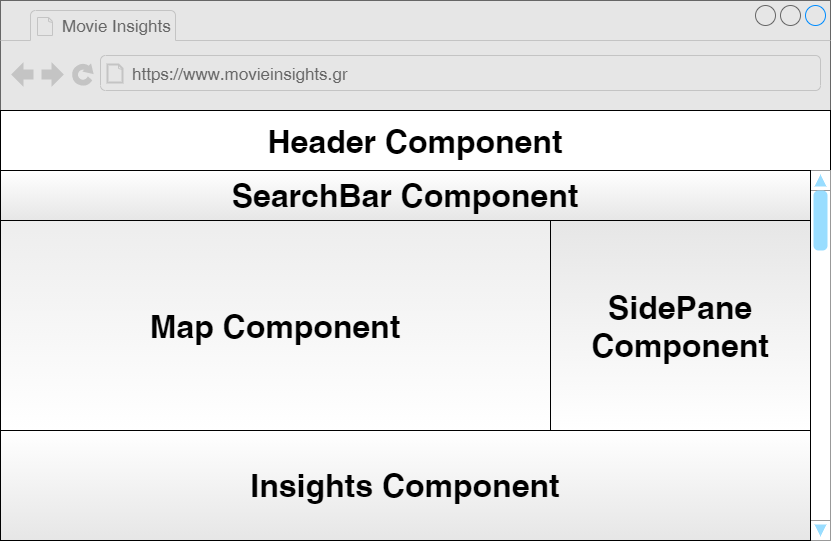
\includegraphics[width=145mm]{Chapters/5 - Architecture/Client/Images/dashboard_struct.png}
  \caption{Βασική διάταξη Web εφαρμογής}
  \label{wire:dashboard}
\end{figure}

Το Dashboard Module ορίζει το δικό του Router που αποτελείται από ένα Route /app/* και ένα RedirectRoute από το κεντρικό Route / στο /app το οποίο είναι η κεντρική σελίδα καθώς δεν χρειάζεται κάτι σύνθετο. 

Ο τρόπος που λειτουργεί είναι ο εξής. Είναι επιλεγμένη για παράδειγμα μια κατηγορία "Στοιχεία για την χώρα Ελλάδα".
Σε αυτήν την κατηγορία στα δεδομένα υπάρχουν οι πιο δημοφιλείς ηθοποιοί, παραγωγοί, σκηνοθέτες, συγγραφείς που έχουν συμμετάσχει σε ταινίες που είτε η παρήγαγε η Ελλάδα είτε η Ελλάδα ήταν χώρα συμπαραγωγής. Αναφέρει επίσης την πιο δημοφιλή εταιρία παραγωγής που συνεργάστηκε η Ελλάδα αλλά και την πιο δημοφιλή χώρα συμπαραγωγής και είδος ταινίας. Επιπρόσθετα αναφέρει τα μέσα και συνολικά έσοδα/έξοδα καθώς και το καθαρό κέρδος. Όλα αυτά τα στοιχεία υπάρχουν επίσης και ανά χρόνο, για όσα χρόνια υπάρχουν στην βάση δεδομένων για την Ελλάδα. Όλες οι κατηγορίες λειτουργούν με τον ίδιο τρόπο με την εξαίρεση της κατηγορίας ανά άτομο. Που εκεί εκτός από την επιλογή χρόνου, υπάρχει και η επιλογή ρόλου, με διαθέσιμους ρόλους: ηθοποιός, σκηνοθέτης, συγγραφέας και παραγωγός. Για τα άτομα υπάρχουν συγκεντρωτικά στοιχεία μόνο ανά ρόλο και όχι συνολικά, καθώς είναι διαφορετικά τα δεδομένα. Πάραυτα όλα τα στοιχεία ανά ρόλο υπάρχουν και ανά χρόνο.

Το Dashboard Module περιέχει μόνο ένα Component το ΜΙDashboard Component. Όλα τα δεδομένα που υπολογίζονται μέσα από το Dashboard Module στέλνονται απευθείας στο ΜΙDashboard Component.

Μέσω των Component που δηλώνονται και δομείται όλη η εφαρμογή καθίσταται εφικτή η πλοήγηση σε όλο το εύρος των δεδομένων της εφαρμογής. Ενώ θα μπορούσε σε κάθε Component, που επηρεάζει τα δεδομένα που εμφανίζονται, να υλοποιηθεί η λογική της αλλαγής των δεδομένων, προτιμήθηκε όλα αυτά τα Component απλά να αλλάζουν την διεύθυνση στην γραμμή διεύθυνσης του Browser και με βάση την διεύθυνση που άλλαξε χωρίς να γίνεται ανακατεύθυνση το Dashboard Module καταλαβαίνει τι χρειάζεται να αλλάξει, αλλάζει τα δεδομένα μέσω του Redux State Manager, και ύστερα στέλνει τα δεδομένα σε όλα τα επιμέρους Components για να αλλάξουν. Ενώ ακούγεται πιο σύνθετη τεχνική, χρησιμοποιήθηκε για την ευκολία διαχείρισης και συντήρησης του κώδικα, καθώς στην άλλη περίπτωση θα έπρεπε σε περίπτωση αλλαγής του κώδικα εμφάνισης των δεδομένων, να πραγματοποιηθούν αλλαγές σε κάθε Component που άλλαζε δεδομένα. Ενώ με αυτήν την υλοποίηση τα πάντα βρίσκονται σε ένα μέρος. Ένας ακόμα σημαντικός λόγος που προτιμήθηκε η συγκεκριμένη τεχνική είναι η προσβασιμότητα στα δεδομένα αυτά. Λόγω της φύσης της αρχιτεκτονικής της εφαρμογής και όντας SPA, υπάρχει ουσιαστικά μόνο μια αληθινή σελίδα που είναι προσβάσιμη από έναν Browser. Αυτή είναι η index.html που είναι ένα αρχείο HTML το οποίο φορτώνει όλον τον κώδικα της εφαρμογής. Χωρίς την αλλαγή της διεύθυνσης, ένας χρήστης θα έπρεπε να μπει στην αρχική σελίδα και να εκτελέσει κάποιες ενέργειες έτσι ώστε να φτάσει στο ίδιο σημείο που βρισκόταν πριν. Με την αλλαγή της διεύθυνσης όμως, όχι μόνο μπορεί να επανέλθει στο σημείο στο οποίο βρισκόταν αλλά μπορεί και να μοιραστεί τον σύνδεσμο με κάποιον άλλον χρήστη και να κοιτάνε τα ίδια δεδομένα. 

Το Dashboard Module λοιπόν παρακολουθεί τις αλλαγές διευθύνσεων που γίνονται μετά την βασική διεύθυνση /app/ και με την χρήση κάποιον βοηθητικών συναρτήσεων αλλάζει τα δεδομένα όπως φαίνεται στον κώδικα \ref{code:urlIntercept}.

\begin{figure}[h]
    \begin{TypeScriptcode}
handleViewChange = () => {
    const path = this.props.location.pathname;
    if (this.state.path !== path || !this.state.pathHandled) {
      if (!this.state.pathHandled) {
        let pathMatch: match;
        if ((pathMatch = matchPath(path, "/app/:entity(country|company|genre)/:id-:name/:year(\\d{4})?"))) {
          this.handleGenericChange(pathMatch.params['entity'], +pathMatch.params['id'], +pathMatch.params['year']);
        } else if ((pathMatch = matchPath(path, "/app/person/:id-:name/:role([A-z]+)?/:year(\\d{4})?"))) {
          this.handlePersonChange(+pathMatch.params['id'], +pathMatch.params['year'], pathMatch.params['role']);
        } else if ((pathMatch = matchPath(path, "/app/:general(general)?/:year(\\d{4})?"))) {
          this.handleGeneralChange(+pathMatch.params['year']);
        }
        this.scrollElement();
        if (this.state.path !== path)
          this.setState({path});
      }
      if (this.state.path !== path) {
        this.setState({pathHandled: false});
      }
    }
}
    \end{TypeScriptcode}
    \caption{Αλγόριθμος παρακολούθησης αλλαγής στην γραμμή διευθύνσεων ενός Browser.}
   \label{code:urlIntercept}
\end{figure}

Η αλλαγή της διεύθυνσης στην γραμμή διευθύνσεων του Browser, δημιουργείται από μια βοηθητική συνάρτηση όπως φαίνεται στον κώδικα \ref{code:urlBuilder}. Με αυτόν τον τρόπο όλα τα Components που έχουν ως σκοπό την αλλαγή των δεδομένων μπορούν να αλλάξουν εύκολα την διεύθυνση χρησιμοποιώντας αυτήν την συνάρτηση, και αν αλλάξει ποτέ η δομή της διεύθυνσης η αλλαγή θα γίνει μόνο μέσα σε αυτήν την συνάρτηση διευκολύνοντας παράλληλα την συντήρηση και την αντιμετώπιση προβλημάτων του κώδικα.

\begin{figure}[h]
    \begin{TypeScriptcode}
function |$\textbf{generateNavigationLink}$|(entity?: BaseNamedEntity, role?: CreditRole, year?: number, entityType?: EntityType) {
  let type = undefined;
  if (entity) {
    if (entityType) {
      type = entityType.toLowerCase();
    } else if (isMovie(entity)) {
      type = 'movie';
    } else if (isPerson(entity)) {
      type = 'person';
    } else if (isCompany(entity)) {
      type = 'company';
    } else if (isCountry(entity)) {
      type = 'country';
    } else if (isGenre(entity)) {
      type = 'genre';
    }
  } else if (year) {
    type = 'general';
  }
  return `/app${type ? `/${type}` : ''}${entity ? `/${entity.id}-${normalizeText(entity.name)}` : ''}${role && type === 'person' ? `/${role}` : ''}${year ? `/${year}` : ''}`;
}
    \end{TypeScriptcode}
    \caption{Αλγόριθμος δημιουργίας διεύθυνσης αλλαγής δεδομένων.}
   \label{code:urlBuilder}
\end{figure}

Το Redux State Manager χρησιμοποιήθηκε για 2 λόγους. Προσφέρει μια εύκολη διεπαφή που βασίζεται στο Immutability των δεδομένων συμβάλλοντας δραστικά στην μείωση των Side Effects, αλλά επίσης χρησιμοποιήθηκε σαν ένα Facade για την απόκτηση των δεδομένων από την υπηρεσία.

Γνωρίζοντάς ότι οποιαδήποτε ενέργεια εμπεριέχει κάποιου είδους επικοινωνία με μια εξωτερική υπηρεσία αυξάνει σημαντικά τον χρόνο της διεκπεραίωσης της, και έχοντας σαν δεδομένο ότι η JavaScript που τρέχει μέσα σε έναν Browser τρέχει σε ένα και μοναδικό νήμα (Thread), η εμπειρία του χρήστη θα ήταν πολύ άσχημη όταν θα ζητούσε νέα δεδομένα από τον Server, καθώς η Web Εφαρμογή θα ήταν μη αποκρίσιμη για αρκετό διάστημα μέχρι την απόκτηση των δεδομένων και την εμφάνιση τους. Για αυτόν τον λόγο χρησιμοποιήθηκε ένα πρόσθετο στο Redux Fraemwork, που επιτρέπει την ασύγχρονη απόκτηση δεδομένων και την αποθήκευση τους στο κεντρικό State της εφαρμογής. Όλα τα Components που εξαρτιούνται από αυτό το Global State, όταν αλλάξει θα αλλάξουν και αυτά τα δεδομένα που εμφανίζουν.

Όπως προαναφέρθηκε το Dashboard Component περιέχει 4 σημαντικά Component που εμφανίζουν όλα τα απαραίτητα δεδομένα.

\subsubsection{SearchBar Component}
Το πρώτο Component μέσα στο MIDashboard Component είναι η γραμμή αναζήτησης, MISearchBar Component. Το MISearchBar Component δεν προσφέρει την δυνατότητα γενικής αναζήτησης αλλά μόνο την δυνατότητα επιλογής ενός αποτελέσματος απο τις προτάσεις της μηχανής αναζήτησης. Οι προτάσεις δημιουργούνται απο την μηχανή αναζήτησης μέσο του Server όπως προαναφέρθηκε νωρίτερα κάθε φορά που ο χρήστης γράφει οποιοδήποτε γράμμα στην μπάρα αναζήτησης όπως φαίνεται στον κώδικα \ref{code:searchbar_suggestion}.

\begin{figure}[H]
    \begin{TypeScriptcode}
async function getSuggestions(value: string): Promise<ACResult[]> {
    const results: AutoComplete = (await Service.search(value)).data;
    return results._
      .map(result => {
        result.e.forEach(e => {
          e.i = result.i
        })
        return result;
      })
      .filter(result => result.e.length > 0);
}
    \end{TypeScriptcode}
    \caption{Αλγόριθμος ανάκτησης προτάσεων αποτελεσμάτων μηχανής αναζήτησης}
   \label{code:searchbar_suggestion}
\end{figure}

Οι προτάσεις της μηχανής αναζήτησης εμφανίζονται με μια μικρή εικόνα στα αριστερά και το κείμενο του αποτελέσματος ακριβώς από διπλά. Ανάλογα με το κείμενο της αναζήτησης που έγραψε ο χρήστης προσπαθεί να υπογραμμίσει με μπλε χρώμα τα γράμματα που βρέθηκαν στα αποτελέσματα όπως φαίνεται στην εικόνα \ref{layout:misearchbar}.
\begin{figure}[H]
  \centering
  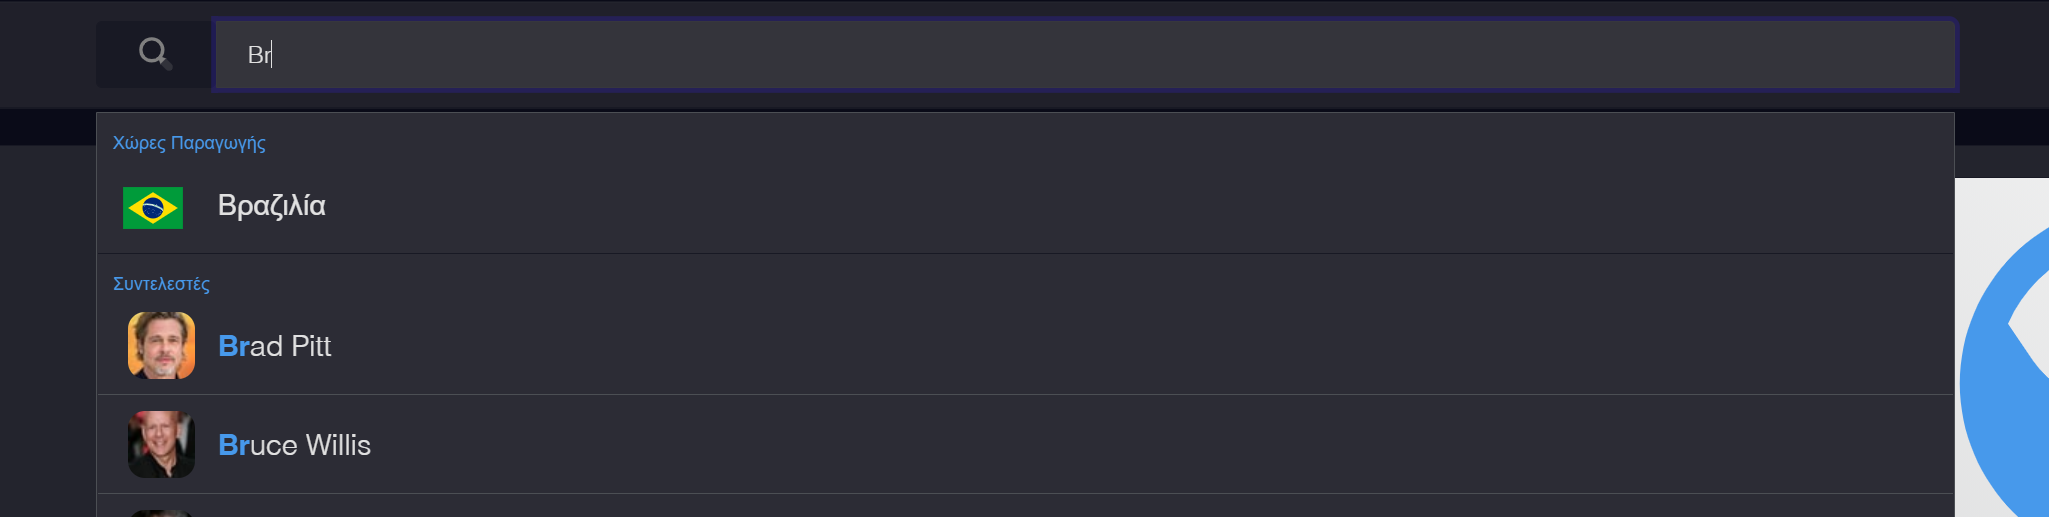
\includegraphics[width=145mm]{Chapters/5 - Architecture/Client/Images/misearchbar_results.png}
  \caption{MISearchBar Component}
  \label{layout:misearchbar}
\end{figure}
Οταν επιλεγεί ενα απο τα προτεινόμενα αποτελέσματα η μπάρα αναζήτησης σβήνει και αλλάζει η διεύθυνση όπως φαίνεται στον κώδικα \ref{code:searchbar_urlchange}

\begin{figure}[H]
    \begin{TypeScriptcode}
private onSearch = (val: ACEntity) => {
  this.props.history.push(AppUtils.|\textbf{generateNavigationLink}|(val, null, null, val.i));
}
    \end{TypeScriptcode}
    \caption{Αλγόριθμος αλλαγής διεύθυνσης απο το MISearchBar Component}
   \label{code:searchbar_urlchange}
\end{figure}

\subsubsection{MapComponent}
Το δεύτερο είναι το Map Component και είναι ένα Component το οποίο προσφέρει ένα προ-ρυθμισμένο Chart από την βιβλιοθήκη Highcharts Highmaps και προσφέρει μια εύκολη διεπαφή για την αλληλεπίδραση και εμφάνιση δεδομένων σε αυτόν τον χάρτη όπως φαίνεται στο σχήμα \ref{layout:mapcomponent}. Κάθε φορά που ο δείκτης του ποντικιού περνάει πάνω απο μια χώρα εμφανίζεται ενα tooltip που γράφει το όνομα της χώρας και σε πόσες ταινίες έχει συμμετάσχει αυτή η χώρα. Όταν πατηθεί μια χώρα θα επιλεγεί εκτός αν ήταν ήδη επιλεγμένη που τότε θα σταματήσει να είναι επιλεγμένη και θα αλλάξει η διεύθυνση όπως φαίνεται στον κώδικα στο σχήμα \ref{code:map_urlchanger}.
\begin{figure}[H]
  \centering
  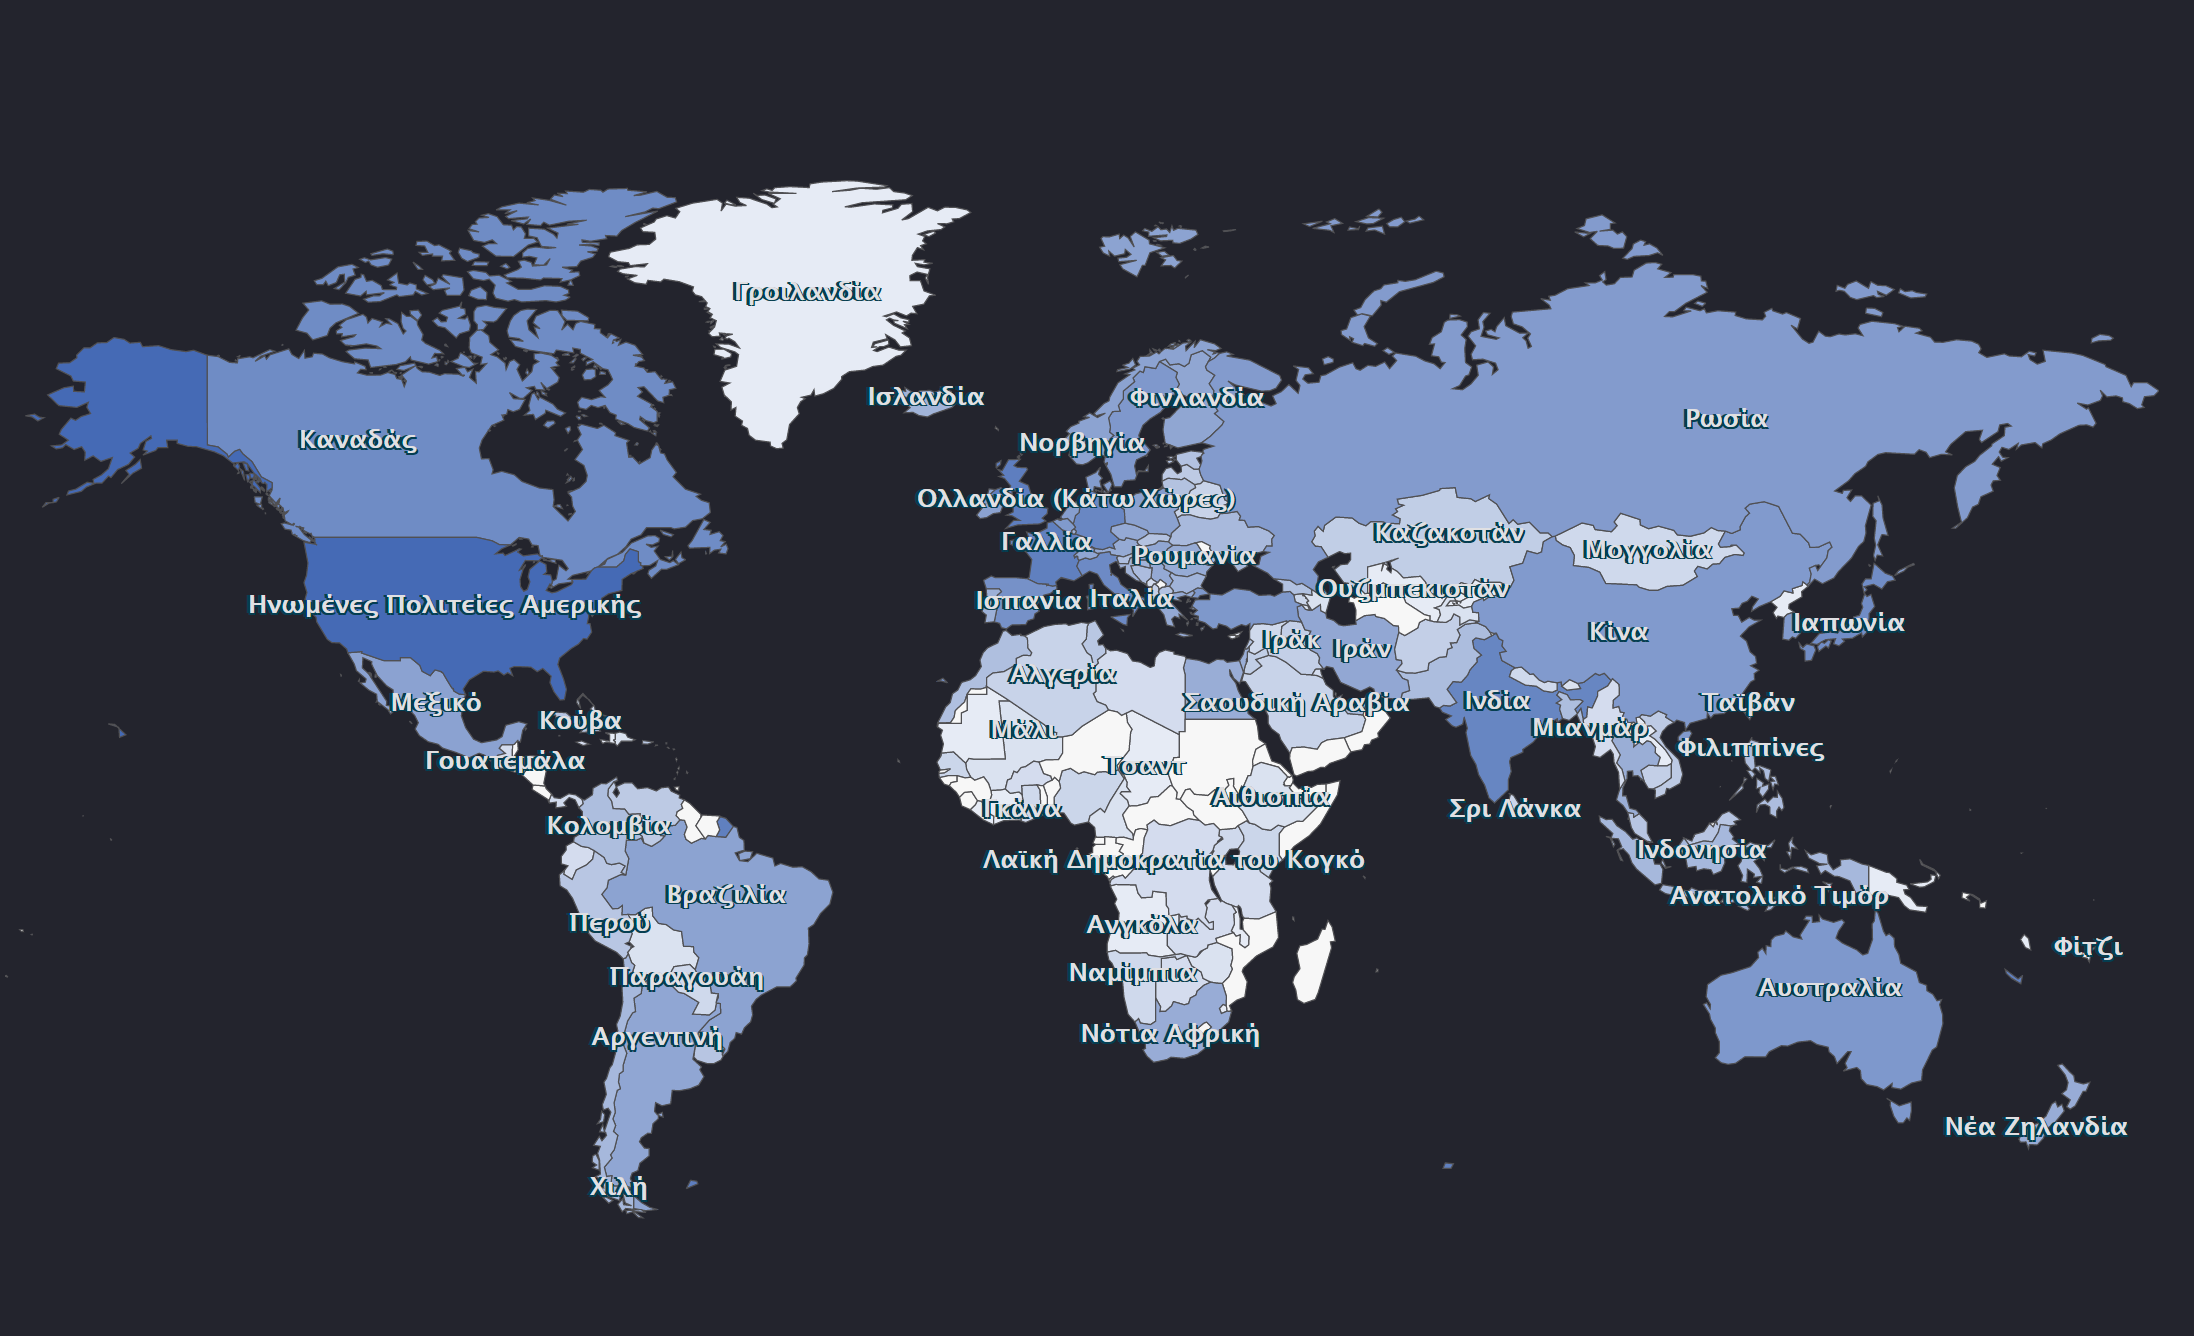
\includegraphics[width=140mm]{Chapters/5 - Architecture/Client/Images/world_map.PNG}
  \caption{Map Component}
  \label{layout:mapcomponent}
\end{figure}

\begin{figure}[H]
    \begin{TypeScriptcode}
countrySelected = (data: ICountryData) => {
  this.props.history.push(AppUtils.|$\textbf{generateNavigationLink}$|({id: data._id, name: data.name, iso31661: data.iso31661, movies: []} as IProductionCountry))
}
countryUnselected = () => {
  this.props.history.push(`/app`)
}
    \end{TypeScriptcode}
    \caption{Αλγόριθμος αλλαγής διεύθυνσης απο το Map Component.}
   \label{code:map_urlchanger}
\end{figure}
\subsubsection{MISidePane Component}
Το ΜΙSidepane Component είναι το τρίτο Component μέσα στο MIDashboard Component και περιέχει το όνομα της κατηγορίας και μια φωτογραφία αν υπάρχει
για παράδειγμα αν είναι η κατηγορία ανά ηθοποιό και ο ηθοποιός ονομαζόταν Νικόλαος Μαυρόπουλος θα εμφάνιζε αυτό το άτομο και την φωτογραφία του αν υπάρχει στην βάση δεδομένων. Περιέχει επίσης ένα Component για την δυνατότητα φιλτραρίσματος των αποτελεσμάτων ανα χρόνο, το MIYearPicker Component, και παρακάτω 4 ίδια Component τύπου MIChartCard για εμφάνιση δεδομένων και γραφημάτων συνδυαστικά. Επί το πλείστον η διάταξη του MISidePane Component παραμένει σταθερή με εξαίρεση την κατηγορία "ανά άτομο" που προστίθεται ένα ακόμα Component το MIRolePicker που δίνει την δυνατότητα φιλτραρίσματος του ρόλου του ατόμου δηλαδή ηθοποιό, σκηνοθέτη, συγγραφέα και παραγωγό.

Το MIChartCard αποτελείται από ένα Grid το οποίο περιέχει ένα γράφημα Highcharts LineChart που στην ουσία είναι ένα γράφημα με μια η περισσότερες γραμμές, ένα εικονίδιο ακριβώς πάνω στο γράφημα περιγραφικό για τι δεδομένα παρουσιάζονται, και δεδομένα από κάτω. Τα δεδομένα του γραφήματος αναπτύσσουν ένα η παραπάνω ποσοτικό πεδίο ανά χρόνο για όσα χρόνια υπάρχουν στην συγκεκριμένη επιλεγμένη κατηγορία, ενώ τα δεδομένα από κάτω εμφανίζουν είτε τα μέγιστα, είτε τα ελάχιστα, είτε τους μέσους όρους των δεδομένων όπως φαίνεται στο σχήμα \ref{layout:michartcard}. Τα γραφήματα των MIChartCard Components όταν φιλτράρεται η κατηγορία ανά χρόνο απενεργοποιούνται, αλλά τα δεδομένα παρακάτω που αναγράφουν μέγιστα ελάχιστα και μέσους όρους παραμένουν και αναφέρονται στο επιλεγμένο έτος για αυτήν την κατηγορία. Δεν υπήρχε ουσιαστικός λόγος τα γραφήματα να έχουν δεδομένα καθώς αυτό που βλέπει ο χρήστης δεν είναι τα συνολικά δεδομένα παρά μόνο του επιλεγμένου έτους.

\begin{figure}[h]
  \centering
  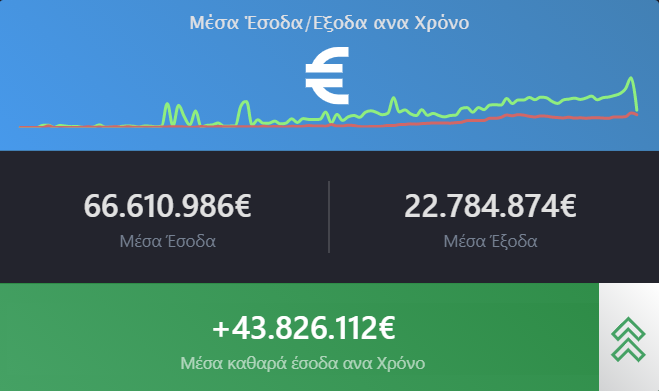
\includegraphics[width=80mm]{Chapters/5 - Architecture/Client/Images/michardcard.png}
  \caption{MIChartCard Component}
  \label{layout:michartcard}
\end{figure}
Το MIYearPicker Component αποτελείται απο 2 κουμπιά και ένα πεδίο εισαγωγής όπως φαίνεται στο σχήμα \ref{layout:miyearpicker}. Όταν πατηθεί το κουμπί με το εικονίδιο ενός ημερολογίου η το πεδίο εισαγωγής, ανοίγει ενα μενού που επιτρέπει την επιλογή ενός έτους που υπάρχει για την επιλεγμένη κατηγορία ενώ οταν πατηθεί το κουμπι με εικονίδιο ενα "Χ" καθαρίζεται η επιλογή του έτους και εμφανίζονται τα συνολικά δεδομένα. Όταν εκτελεστεί μια ενέργεια απο αυτο το Component, θα αλλάξει την διεύθυνση έτσι ώστε να αναλάβει το Dashboard Module την αλλαγή των δεδομένων όπως φαίνεται στον κώδικα \ref{code:miyearpicker_urlchanger}.
\begin{figure}[h]
  \centering
  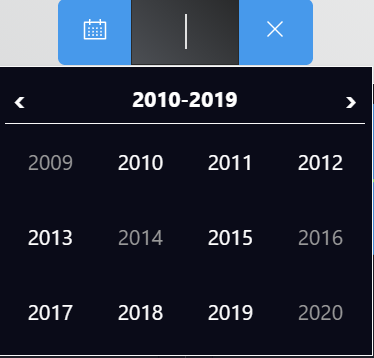
\includegraphics[width=35mm]{Chapters/5 - Architecture/Client/Images/miyearpicker.png}
  \caption{MIYearPicker Component}
  \label{layout:miyearpicker}
\end{figure}

\begin{figure}[h]
    \begin{TypeScriptcode}
yearSelected = (year: number) => {
  const activeView = this.props.rootState.dashboardState.activeView();
  const activeEntity = this.props.rootState.dashboardState.activeView().activeEntity;
  let role = null;
  if (activeView.entityType === EntityType.PERSON) {
    const _activeView = activeView as MovieInsightsPerPersonState;
    role = _activeView.activeRole;
  }
  this.props.history.push(AppUtils.|$\textbf{generateNavigationLink}$|(activeEntity.entity, role, year))
}
yearUnselected = () => {
  const activeEntity = this.props.rootState.dashboardState.activeView().activeEntity;
  if (activeEntity.entity) {
    this.props.history.push(AppUtils.|$\textbf{generateNavigationLink}$|(activeEntity.entity));
  } else {
    this.props.history.push(`/app`);
  }
}
    \end{TypeScriptcode}
    \caption{Αλγόριθμος αλλαγής διεύθυνσης απο το MIYearPicker Component.}
   \label{code:miyearpicker_urlchanger}
\end{figure}
Το MIRolePicker Component εμφανίζεται μόνο όταν η επιλεγμένη κατηγορία είναι "ανά άτομο". Αποτελείται από 4 κουμπιά μονής επιλογής. Αυτό σημαίνει ότι όταν πατηθεί ένα κουμπί επιλέγεται μένει πατημένο και οποιαδήποτε άλλο κουμπί ήταν πατημένο πρωτύτερα αφαιρείται η επιλογή του. Λειτουργεί ακριβώς με τον ίδιο τρόπο με τα παραδοσιακά Radio Buttons. Τα 4 κουμπιά αντιστοιχούν στους 4 ρόλους που μπορεί να έχει ένα άτομο όπως Ηθοποιός, Σκηνοθέτης, Συγγραφέας και Παραγωγός όπως φαίνεται στο σχήμα \ref{layout:mirolepicker}. Όταν ένα Role είναι επιλεγμένο το ανάλογο κουμπί επιλέγεται και εμφανίζεται με χρώμα μπλε, όταν δεν υπάρχει το συγκεκριμένο Role στο άτομο είναι απενεργοποιημένο και εμφανίζεται με χρώμα ανοιχτό γκρι, και αν υπάρχει και δεν είναι επιλεγμένο εμφανίζεται με χρώμα σκούρο γκρι και ο κώδικας επιλογής φαίνεται στο σχήμα. Όταν αλλάζει η επιλογή ο κώδικας που αλλάζει την διεύθυνση φαίνεται στο σχήμα \ref{code:mirolepicker_urlchanger}.
\begin{figure}[h]
  \centering
  
\includegraphics[width=55mm]{Chapters/5 - Architecture/Client/Images/mirolepicker.png}
  \caption{MIRolePicker Component}
  \label{layout:mirolepicker}
\end{figure}

\begin{figure}[H]
    \begin{TypeScriptcode}
private onCreditSelect = (credit: CreditRole) => {
  const activeView = this.props.rootState.dashboardState.activeView() as MovieInsightsPerPersonState;
  this.props.history.push(AppUtils.|$\textbf{generateNavigationLink}$|(activeView._activeEntity.person, credit, activeView.isPerYear ? activeView.activeYearEntity.entity : null));
}
    \end{TypeScriptcode}
    \caption{Αλγόριθμος αλλαγής διεύθυνσης από το MIRolePicker Component.}
   \label{code:mirolepicker_urlchanger}
\end{figure}



\subsubsection{MIInsightsPanel Component}
Το MIInsightsPanel Component είναι το τέταρτο και τελευταίο Component που βρίσκεται μέσα στο MIDashboard Component.
Περιέχει πολλά Component ίδιου τύπου MICard Component. Το κάθε MICard Component είναι μια "κάρτα" που εμφανίζει ένα στοιχείο για ένα άτομο, μια ταινία, μια εταιρία παραγωγής, μια χώρα παραγωγής η ένα είδος ταινίας. Για παράδειγμα αν μια κάρτα για μια ταινία με τα μεγαλύτερα έσοδα θα εμφανιζόταν όπως στο σχήμα \ref{layout:micard_revenue}.

\begin{figure}[h]
  \centering
  
\includegraphics[width=50mm]{Chapters/5 - Architecture/Client/Images/micard_revenue.png}
  \caption{MICard Component}
  \label{layout:micard_revenue}
\end{figure}

Το MICard Component είναι ένα Component το οποιο έχει σχεδιαστεί με ρευστή διάταξη και δυναμικό περιεχόμενο. Ανάλογα με το τι περιεχόμενο θα του δοθεί θα αλλάξει την διάταξη του και θα εμφανίσει τα ανάλογα δεδομένα. Υποστηρίζει Placeholders για την αναμονή των απομακρυσμένων δεδομένων εμφανίζοντας ένα Spinner, και υποστηρίζει και την εμφάνιση ενός μηνύματος λάθους σε περίπτωση που τα δεδομένα για την συγκεκριμένη κατηγορία δεν υπάρχουν. Επιπρόσθετα κάθε Component τυπου MICard μπορεί να πατηθεί σαν κουμπί και ανάλογα με το περιεχόμενο αλλάζει την διεύθυνση στην γραμμή διεύθυνσης του Browser, έτσι ώστε να εμφανιστούν τα ανάλογα δεδομένα μετέπειτα απο το Dashboard Module. Όλα τα MICard λειτουργούν με τον ίδιο τρόπο εκτός απο το MICard που περιέχει δεδομένα ταινιών. Καθώς ο ρόλος της εφαρμογής δεν είναι να εμφανίζει αναλυτικά στοιχεία για ταινίες επειδή υπάρχουν ήδη πολυ γνωστές υπηρεσίες για αυτόν τον σκοπό όπως προαναφέρθηκαν το IMDb και το TMDb, όταν πατηθεί ένα MICard με περιεχόμενο ταινιών θα εμφανιστεί ενα παράθυρο πάνω απο την εφαρμογή το οποίο είναι το MIMovieInfoModal Component όπως φαίνεται στον κώδικα \ref{code:micard_click}.
\begin{figure}[H]
    \begin{TypeScriptcode}
|\textbf{renderCardLinked}|() {
  const link = this.state.entity?AppUtils.|\textbf{generateNavigationLink}|(this.state.entity):''
  return (<NavLink className="mi-card-link" onClick={this.onLinkClick} to={link}>{this.renderCard()}|</NavLink>|);
}
_render() {
  return (
    <>
      {this.state.loaded && this.state.entity ?this.|\textbf{renderCardLinked}|() : this.renderCard()}
      {this.props.entityType === TmdbEntityType.MOVIE ?(|\textbf{<MIMovieInfoModal}| open={this.state.modal} onClose={() => this.setState({modal: false})} entity={this.props.entity as any}|\textbf{/>}|) : null}
    |</>|
  )
}
    \end{TypeScriptcode}
    \caption{Αλγόριθμος αλλαγής διεύθυνσης από το MIRolePicker Component.}
   \label{code:micard_click}
\end{figure}


Το MIMovieInfoModal Component περιέχει το πόστερ της ταινίας καθώς και μια εικόνα background σχετική με την ταινία και περιέχει τα πολύ βασικά στοιχεία που χρησιμοποιεί η εφαρμογή όπως, τα έσοδα, τα έξοδα, την βαθμολογία με της ψήφους της ταινίας καθώς και το πόσο διαρκεί η ταινία συνολικά. Επιπρόσθετα δίνει την επιλογή για περισσότερα στοιχεία για αυτήν την ταινία προσφέροντας 2 συνδέσμους ανακατεύθυνσης που ο ένας πηγαίνει τον χρήστη στον ισότοπο του TMDb στην επιλεγμένη ταινία και ο άλλος στο IMDB όπως φαίνεται στο σχήμα \ref{layout:mimoviemodal}

\begin{figure}[H]
  \centering
  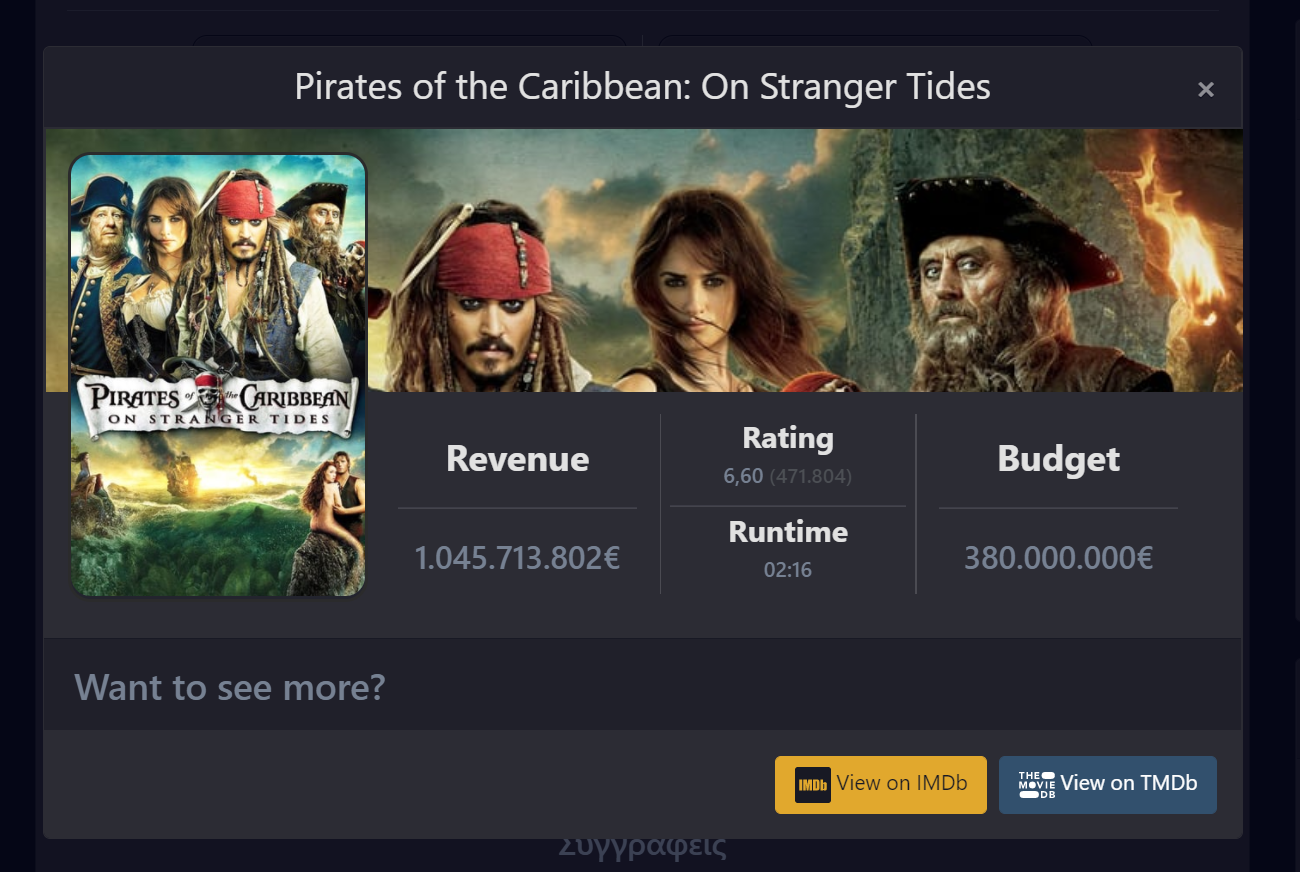
\includegraphics[width=100mm]{Chapters/5 - Architecture/Client/Images/mimoviemodal.png}
  \caption{MIMovieInfoModal Component}
  \label{layout:mimoviemodal}
\end{figure}
\subsection{Admin Module}
Το Admin Module είναι ένα σύνολο λειτουργιών που επιτρέπει έναν διαχειριστή να διαχειρίζεται με ευκολία την εφαρμογή. Στην παρούσα υλοποίηση το Admin Module έχει 2 διαφορετικές σελίδες - Components, το Κέντρο Ελέγχου και το Κέντρο Διαχείρισης Καταγραφών. Για να αποκτήσει πρόσβαση ένας χρήστης στις λειτουργίες του Admin Module, πρέπει να έχει κάνει Login και να είναι εξουσιοδοτημένος με τον ρόλο ADMIN, διαχειριστή. 

Το Κέντρο Ελέγχου είναι μια σελίδα που επιτρέπει την παρακολούθηση της κατάστασης της υγείας της εφαρμογής, προσφέρει στατιστικά των υπηρεσιών αλλά και του λειτουργικού που τρέχει η εφαρμογή αλλα παράλληλα προσφέρει και διαγνωστικά για να γνωρίζει ο διαχειριστής τι γίνεται ανά πάσα στιγμή στην εφαρμογή αυτήν όπως φαίνεται στις εικόνες \ref{layout:admin_cc_1} και \ref{layout:admin_cc_2}. 

Αποτελείται από πολλά διαφορετικά Components τα οποία ενημερώνονται ανάλογα με τον τύπο των δεδομένων που προσφέρουν ανά μισό, δύο και ανά πέντε δευτερόλεπτα με την χρήση WebSockets μέσο του Spring Boot Actuator έτσι ώστε η εικόνα που βλέπει ο διαχειριστής να αντικατοπτρίζει πάντα την κατάσταση της εφαρμογής εκείνη την χρονική στιγμή.

Το Κέντρο Διαχείρισής Καταγραφών είναι στην ουσία ένας διαδραστικός πίνακας που επιτρέπει στον διαχειριστή να αλλάζει τα επίπεδα καταγραφής διάφορων υπηρεσιών μέσα στον Server. Τα επίπεδα καταγραφής ορίζουν τι πληροφορίες θα δίνει η κάθε υπηρεσία. Το επίπεδο καταγραφής ERROR για παράδειγμα καταγράφει μόνο τα μηνύματα σφαλμάτων στο αρχείο καταγραφής της υπηρεσίας, ενώ το επίπεδο καταγραφής WARNING καταγράφει και τα μηνύματα σφαλμάτων αλλά και τα μηνύματα προειδοποιήσεων. Αυτό είναι πολύ χρήσιμο όταν χρησιμοποιείται σε συνδυασμό με μια υπηρεσία διαχείρισης καταγραφών όπως η Logstash για παράδειγμα. Με αυτόν τον τρόπο ο διαχειριστής δεν χρειάζεται να έχει φυσική πρόσβαση στο μηχάνημα που τρέχει την εφαρμογή για να μπορεί να δει τα αρχεία καταγραφής παρά μόνο να μπει στην υπηρεσία διαχείρισης καταγραφών και να βρει ότι χρειάζεται από εκεί.

Ο πίνακας του Κέντρου Διαχείρισής Καταγραφών φαίνεται στην εικόνα \ref{layout:admin_l}. Η συγκεκριμένη εικόνα τραβήχτηκε κατά την ανάπτυξη της εφαρμογής και δείχνει ότι το κεντρικό επίπεδο καταγραφών ROOT είναι ορισμένο στο DEBUG που σημαίνει ότι καταγράφει ακόμα και μηνύματα διαγνωστικών με κάποιες εξαιρέσεις που έχουν οριστεί σε επίπεδο WARNING για να μην υπερφορτώσουν τα αρχεία καταγραφής με περιττές πληροφορίες.

\begin{figure}[H]
  \centering
  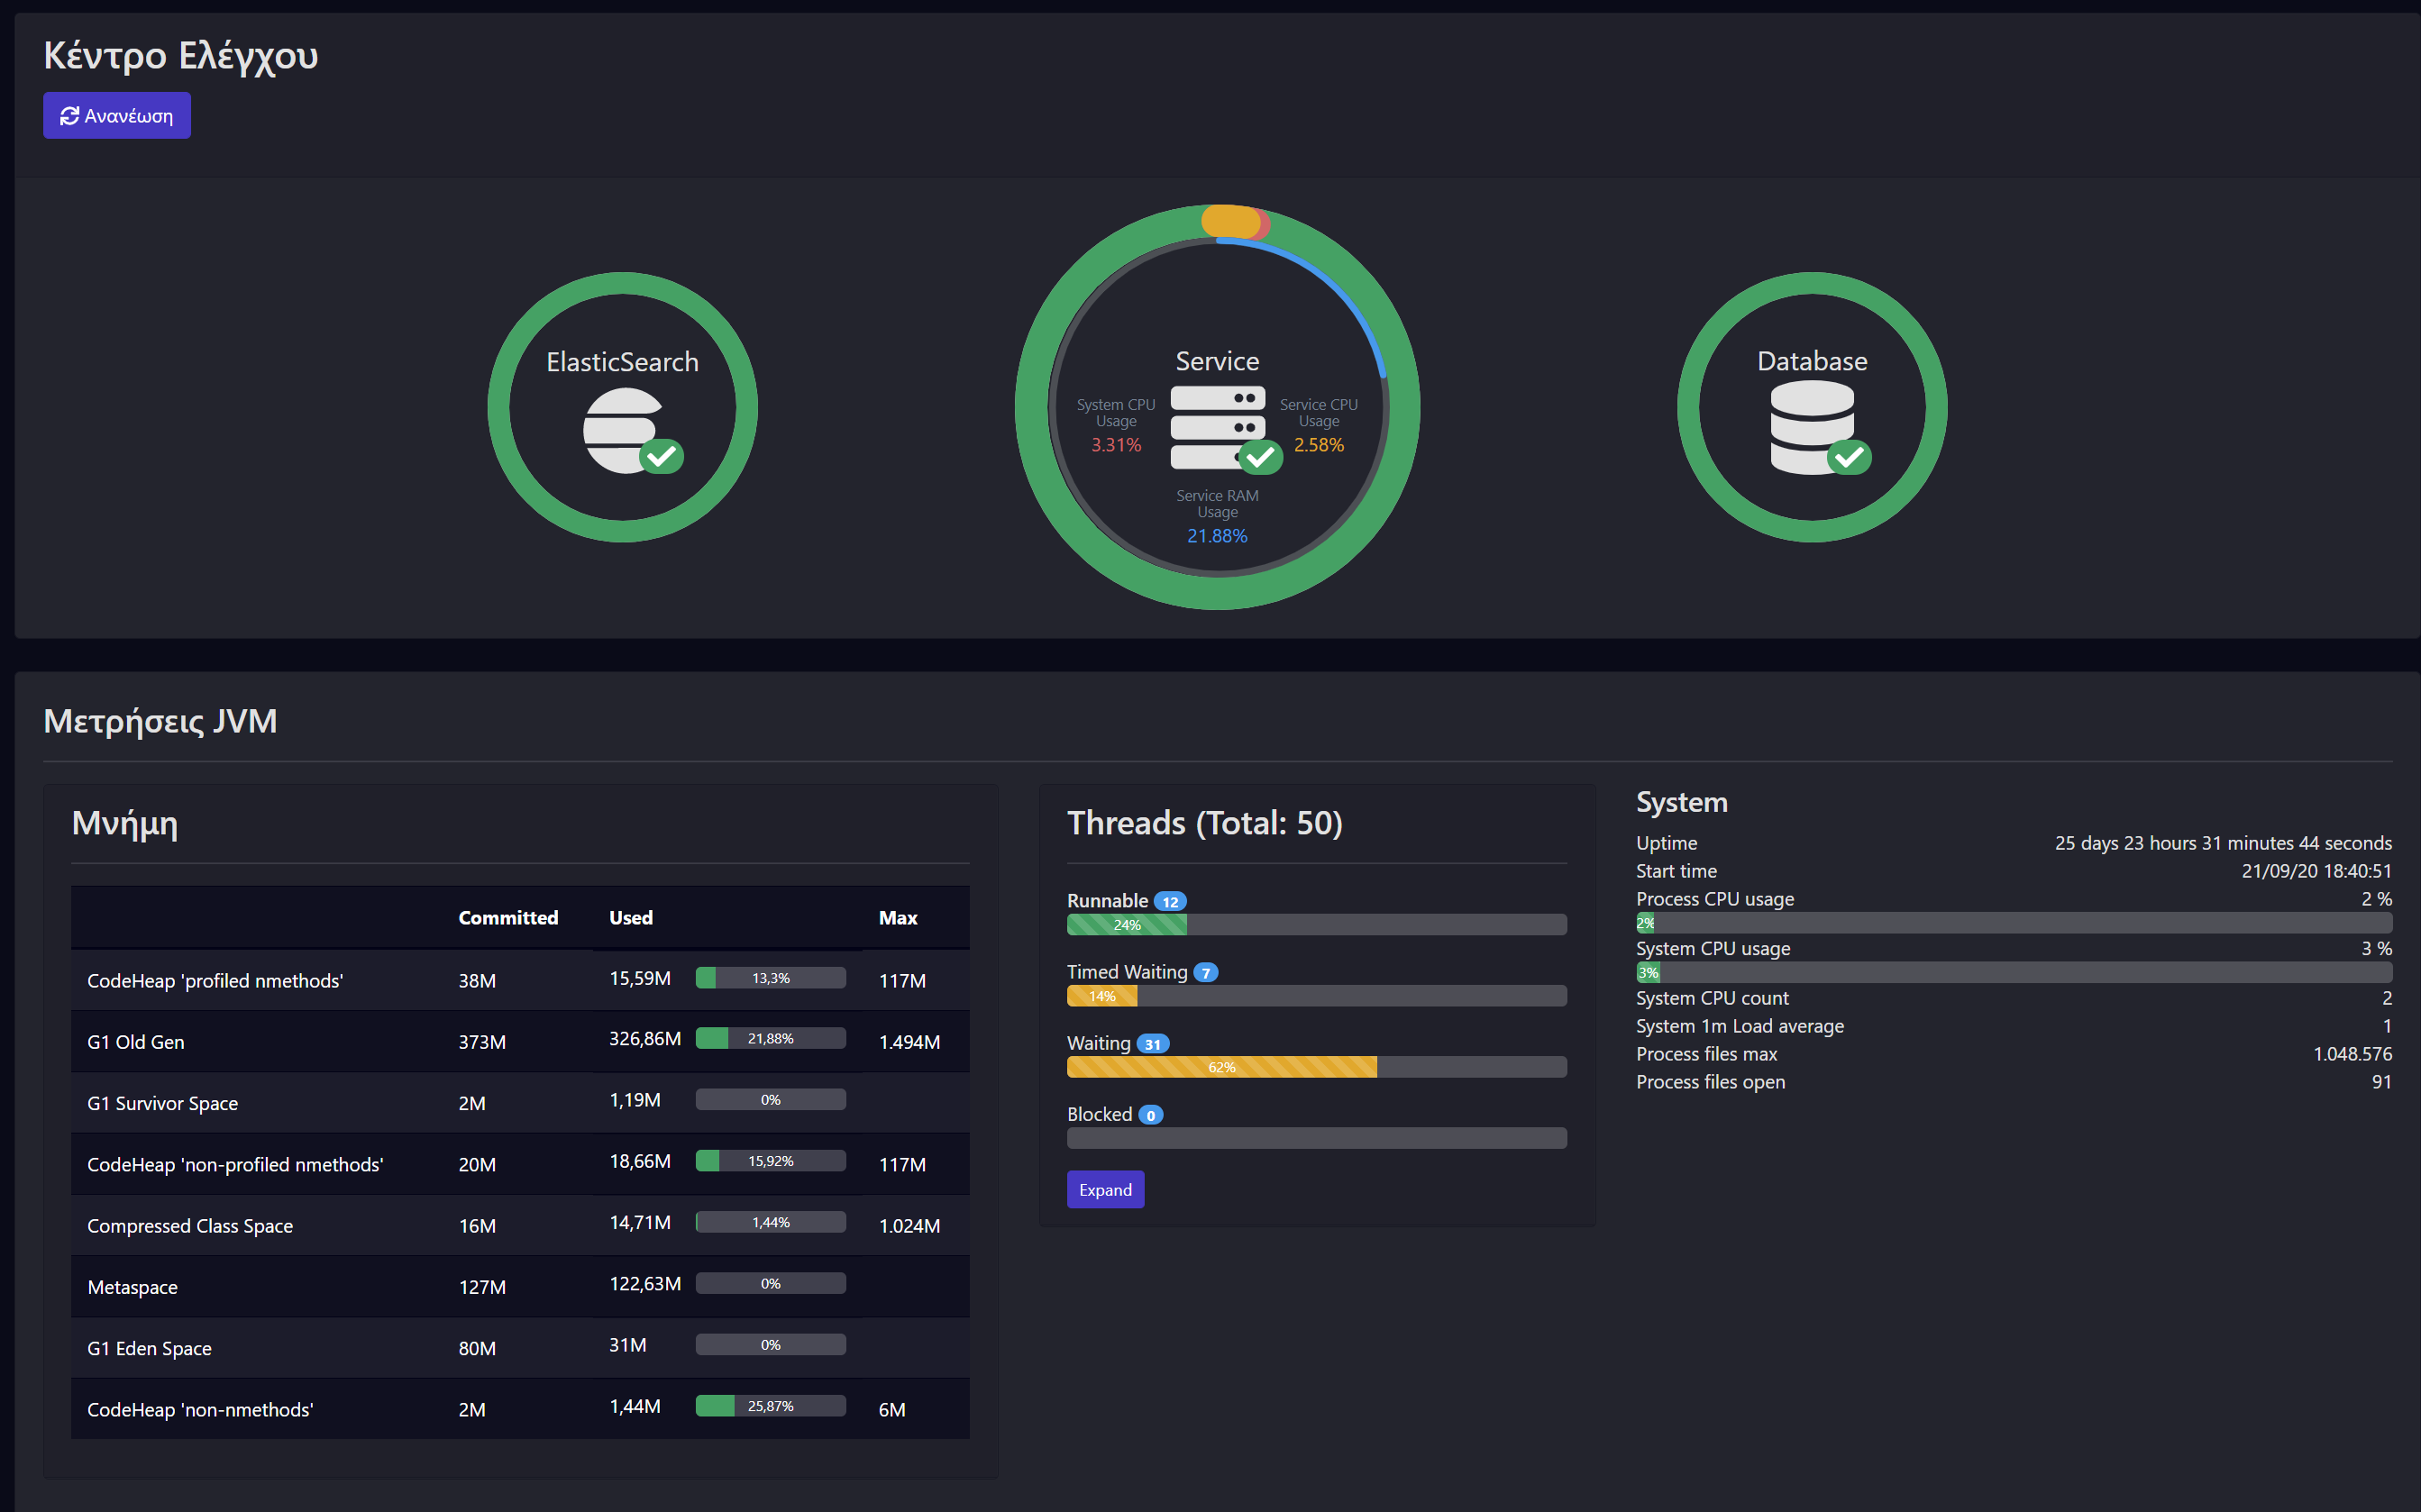
\includegraphics[width=145mm]{Chapters/5 - Architecture/Client/Images/admin_control_center.png}
  \caption{Κέντρο Ελέγχου}
  \label{layout:admin_cc_1}
\end{figure}
\begin{figure}[H]
  \centering
  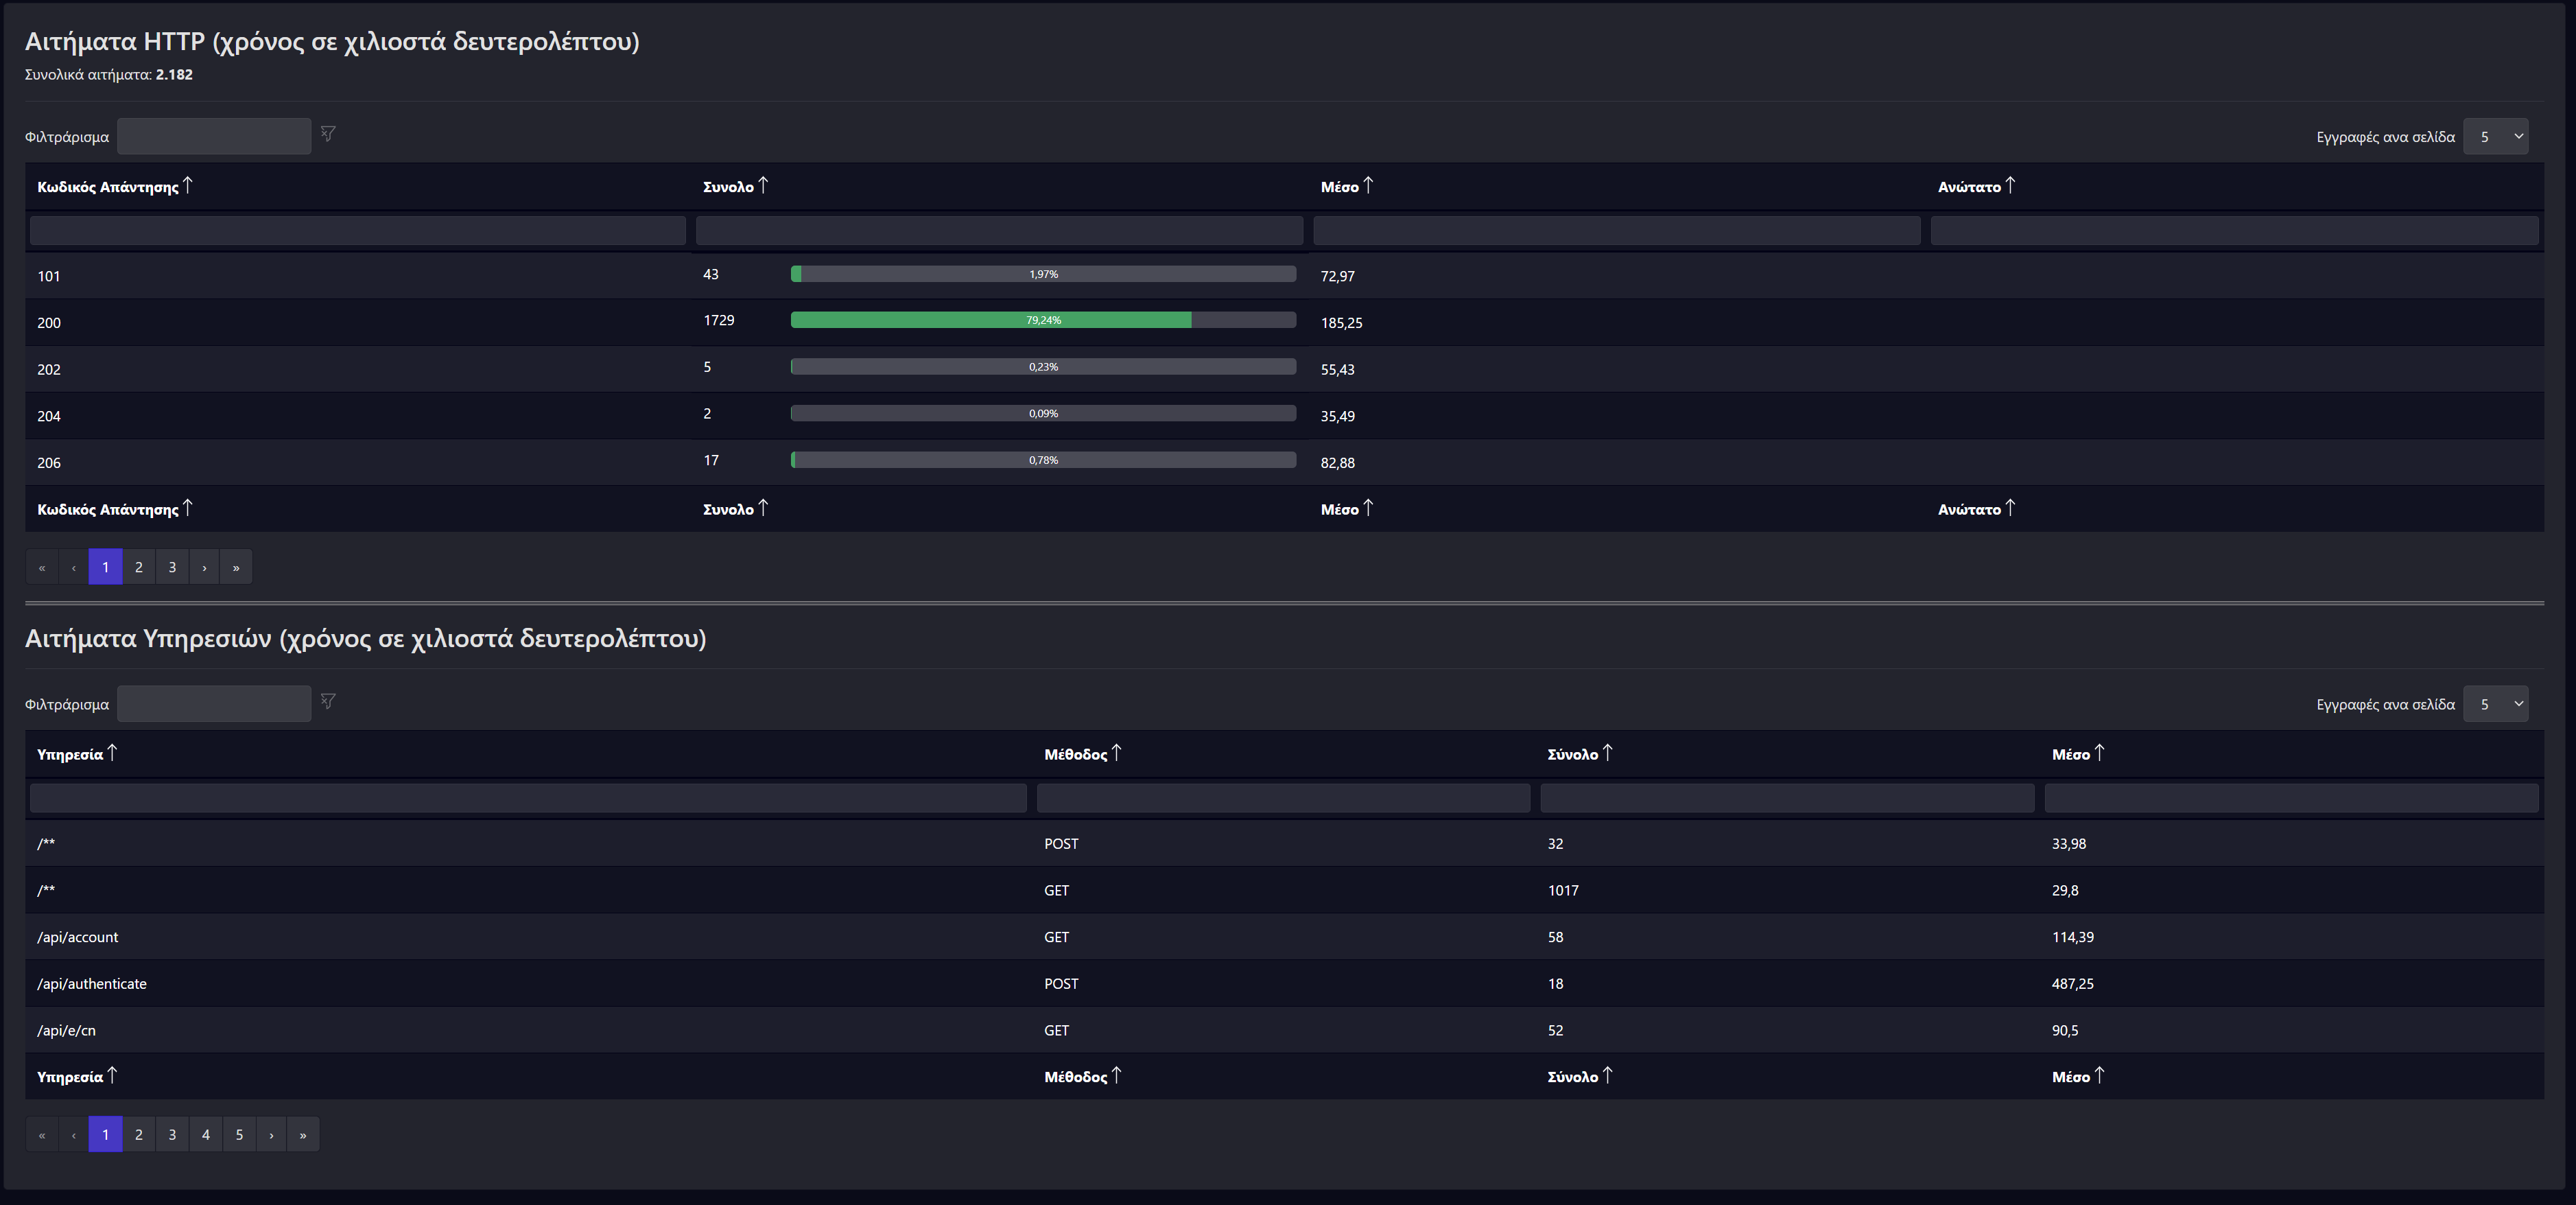
\includegraphics[width=145mm]{Chapters/5 - Architecture/Client/Images/admin_control_center_2.png}
  \caption{Κέντρου Ελέγχου - συνέχεια}
  \label{layout:admin_cc_2}
\end{figure}
\begin{figure}[H]
  \centering
  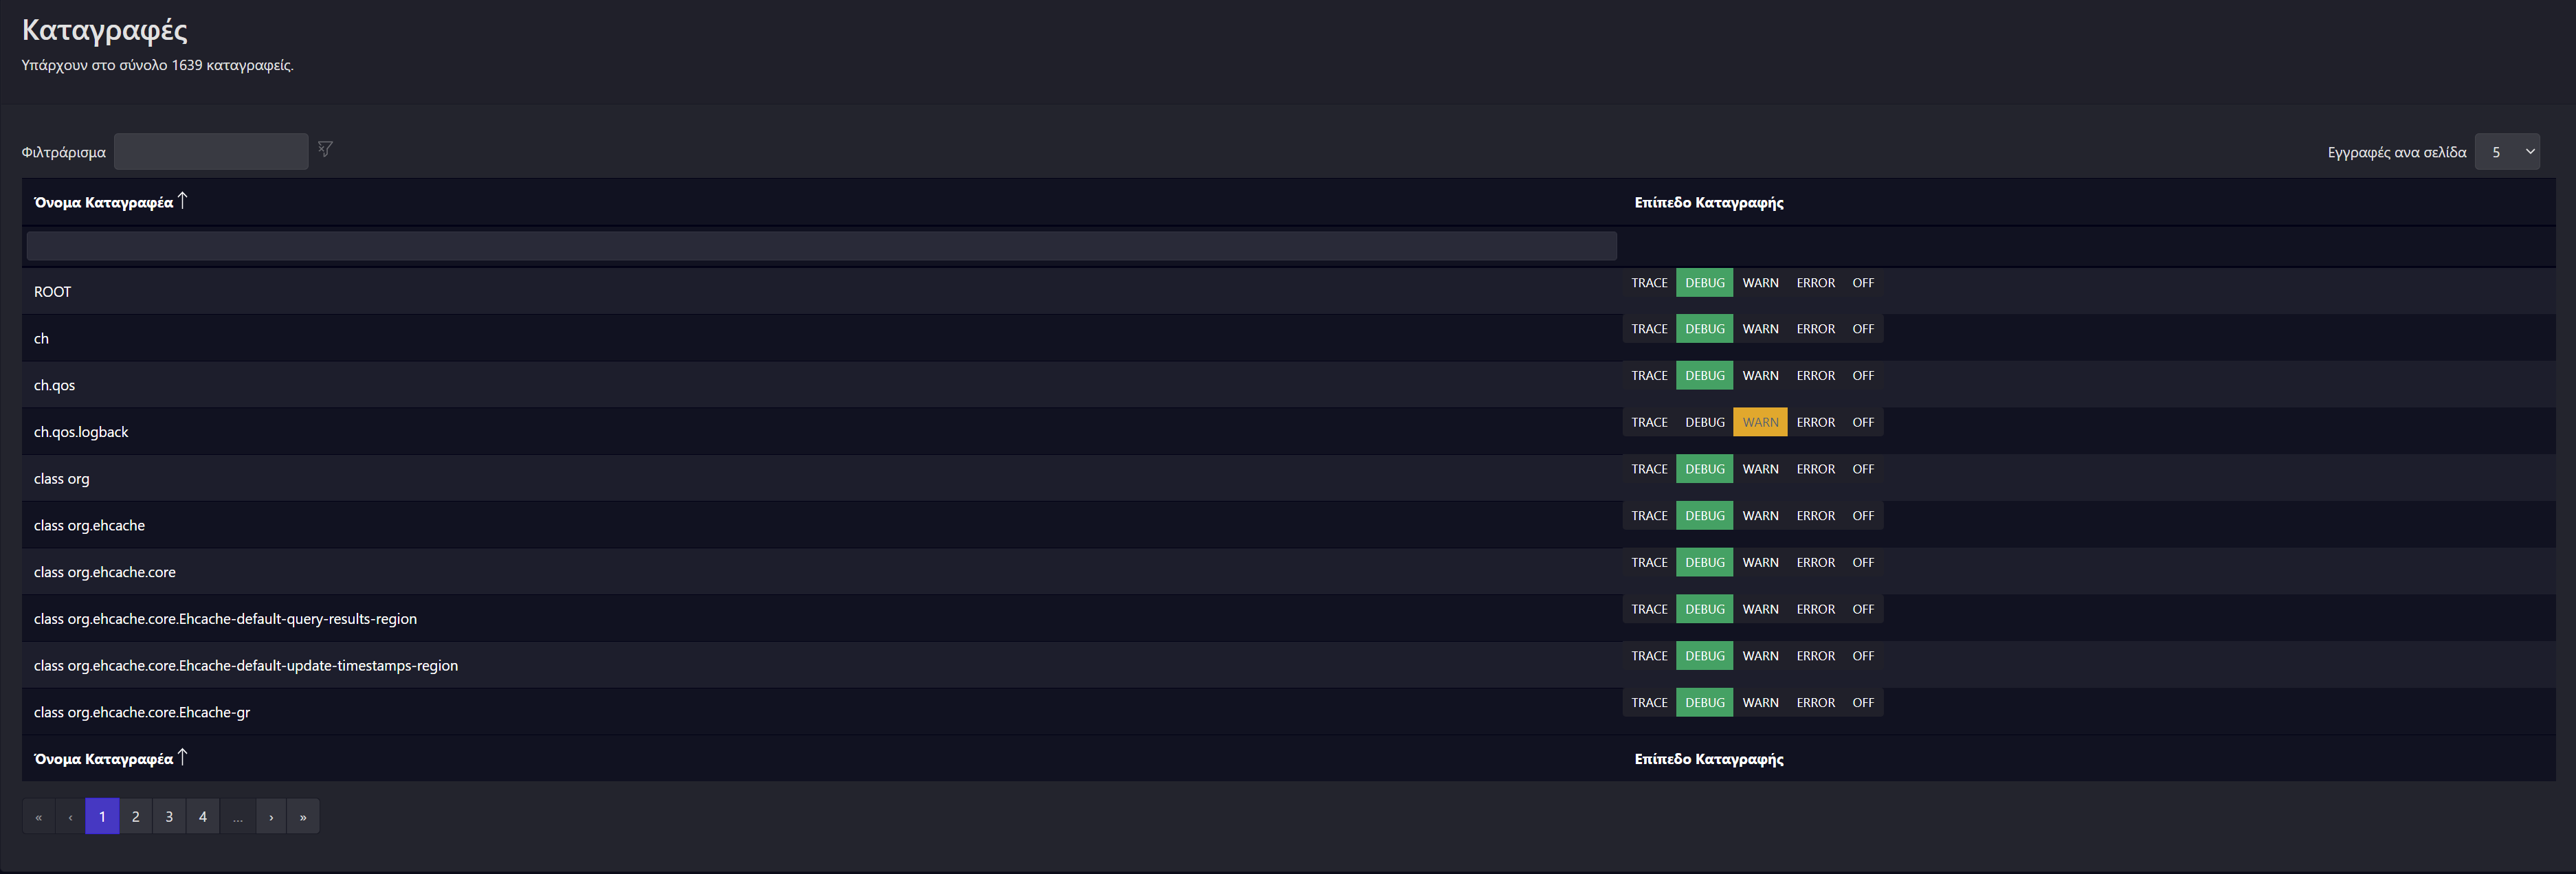
\includegraphics[width=145mm]{Chapters/5 - Architecture/Client/Images/admin_l.png}
  \caption{Κέντρο Διαχείρισής Καταγραφών}
  \label{layout:admin_l}
\end{figure}